\chapter{System Design and Architecture}

\section{Use Case Diagram}
\begin{figure}[ht]
  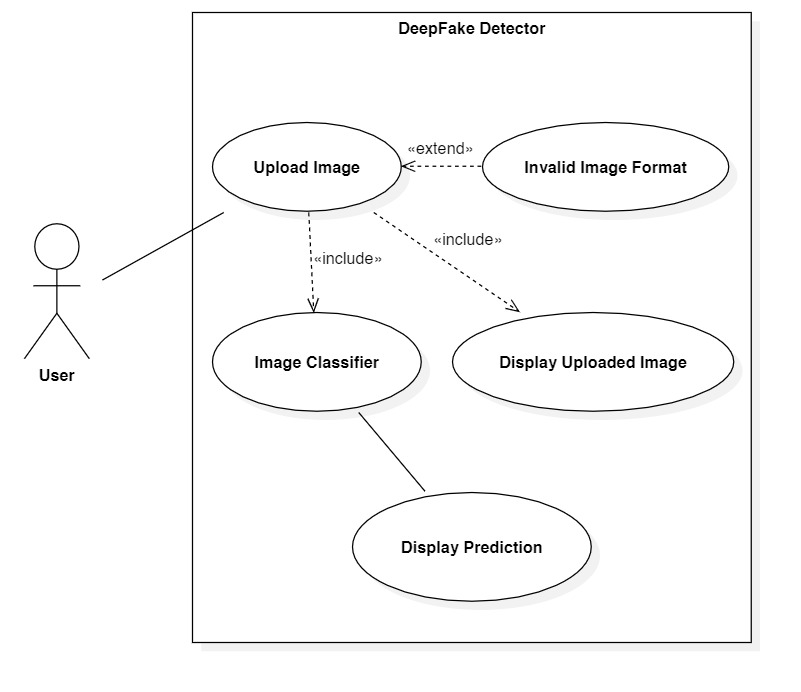
\includegraphics[width=1\textwidth]{./img/UseCaseDiagram.jpg}
  \caption{Use Case Diagram}
\end{figure}

\pagebreak

\section{Sequence Diagram}
\begin{figure}[ht]
  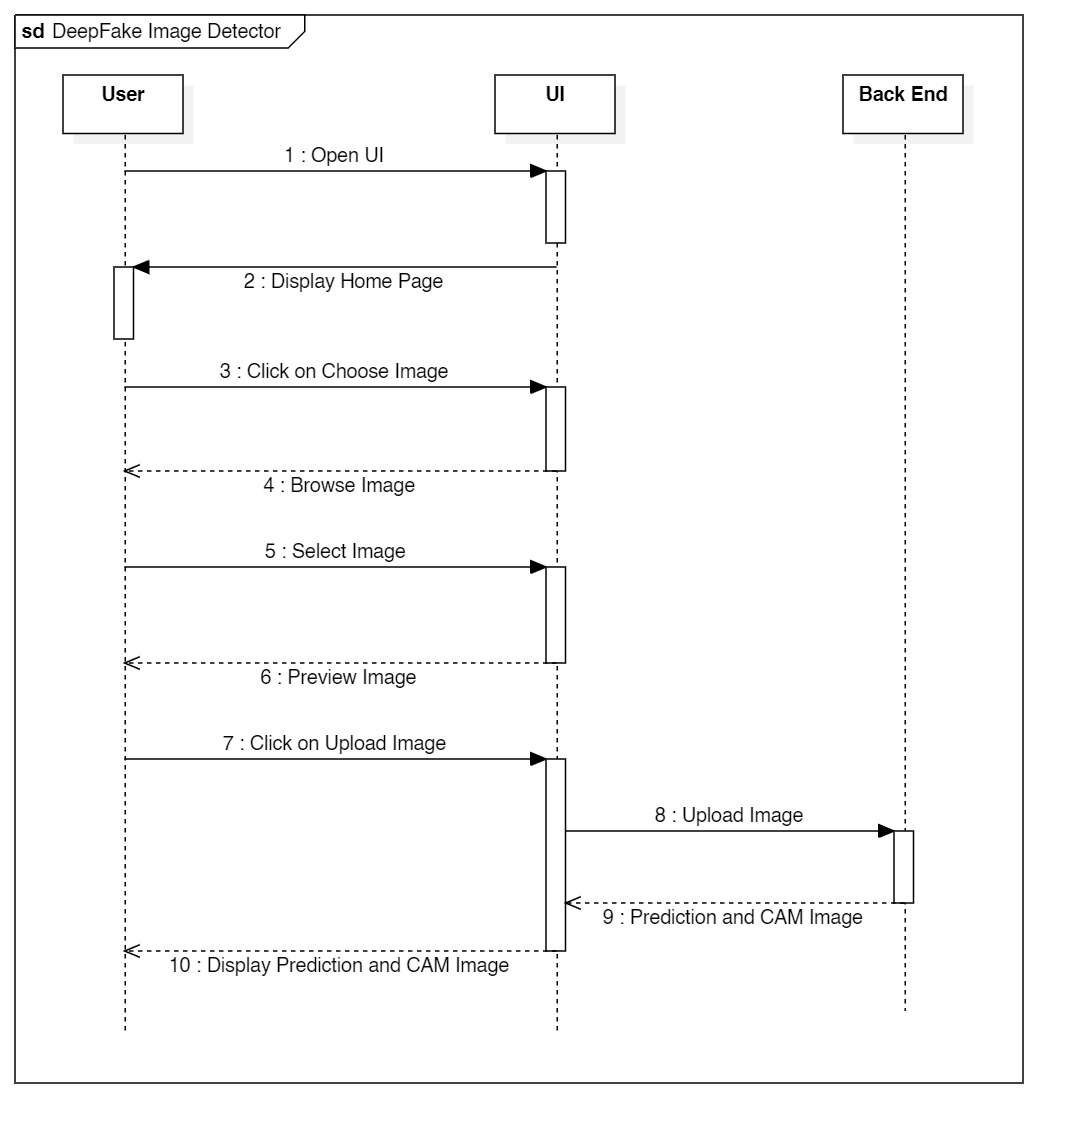
\includegraphics[width=1\textwidth]{./img/sequence diagram.jpg}
  \caption{Sequence Diagram}
\end{figure}

\pagebreak
\section{Proposed System}
Below is the representation of our proposed system, illustrated in Figure 4.4. Initially, we assembled the dataset, as outlined in the Data Collection section above. The dataset was categorized into two groups: real and fake. Subsequently, preprocessing of the data was carried out. For feature extraction and classification, we employed a pre-trained ResNet 9 model. Upon completing the training of the model, it was integrated with a frontend (User Interface) using an API.
\vspace{20pt}
\begin{figure}[hbt!]
    \center{
        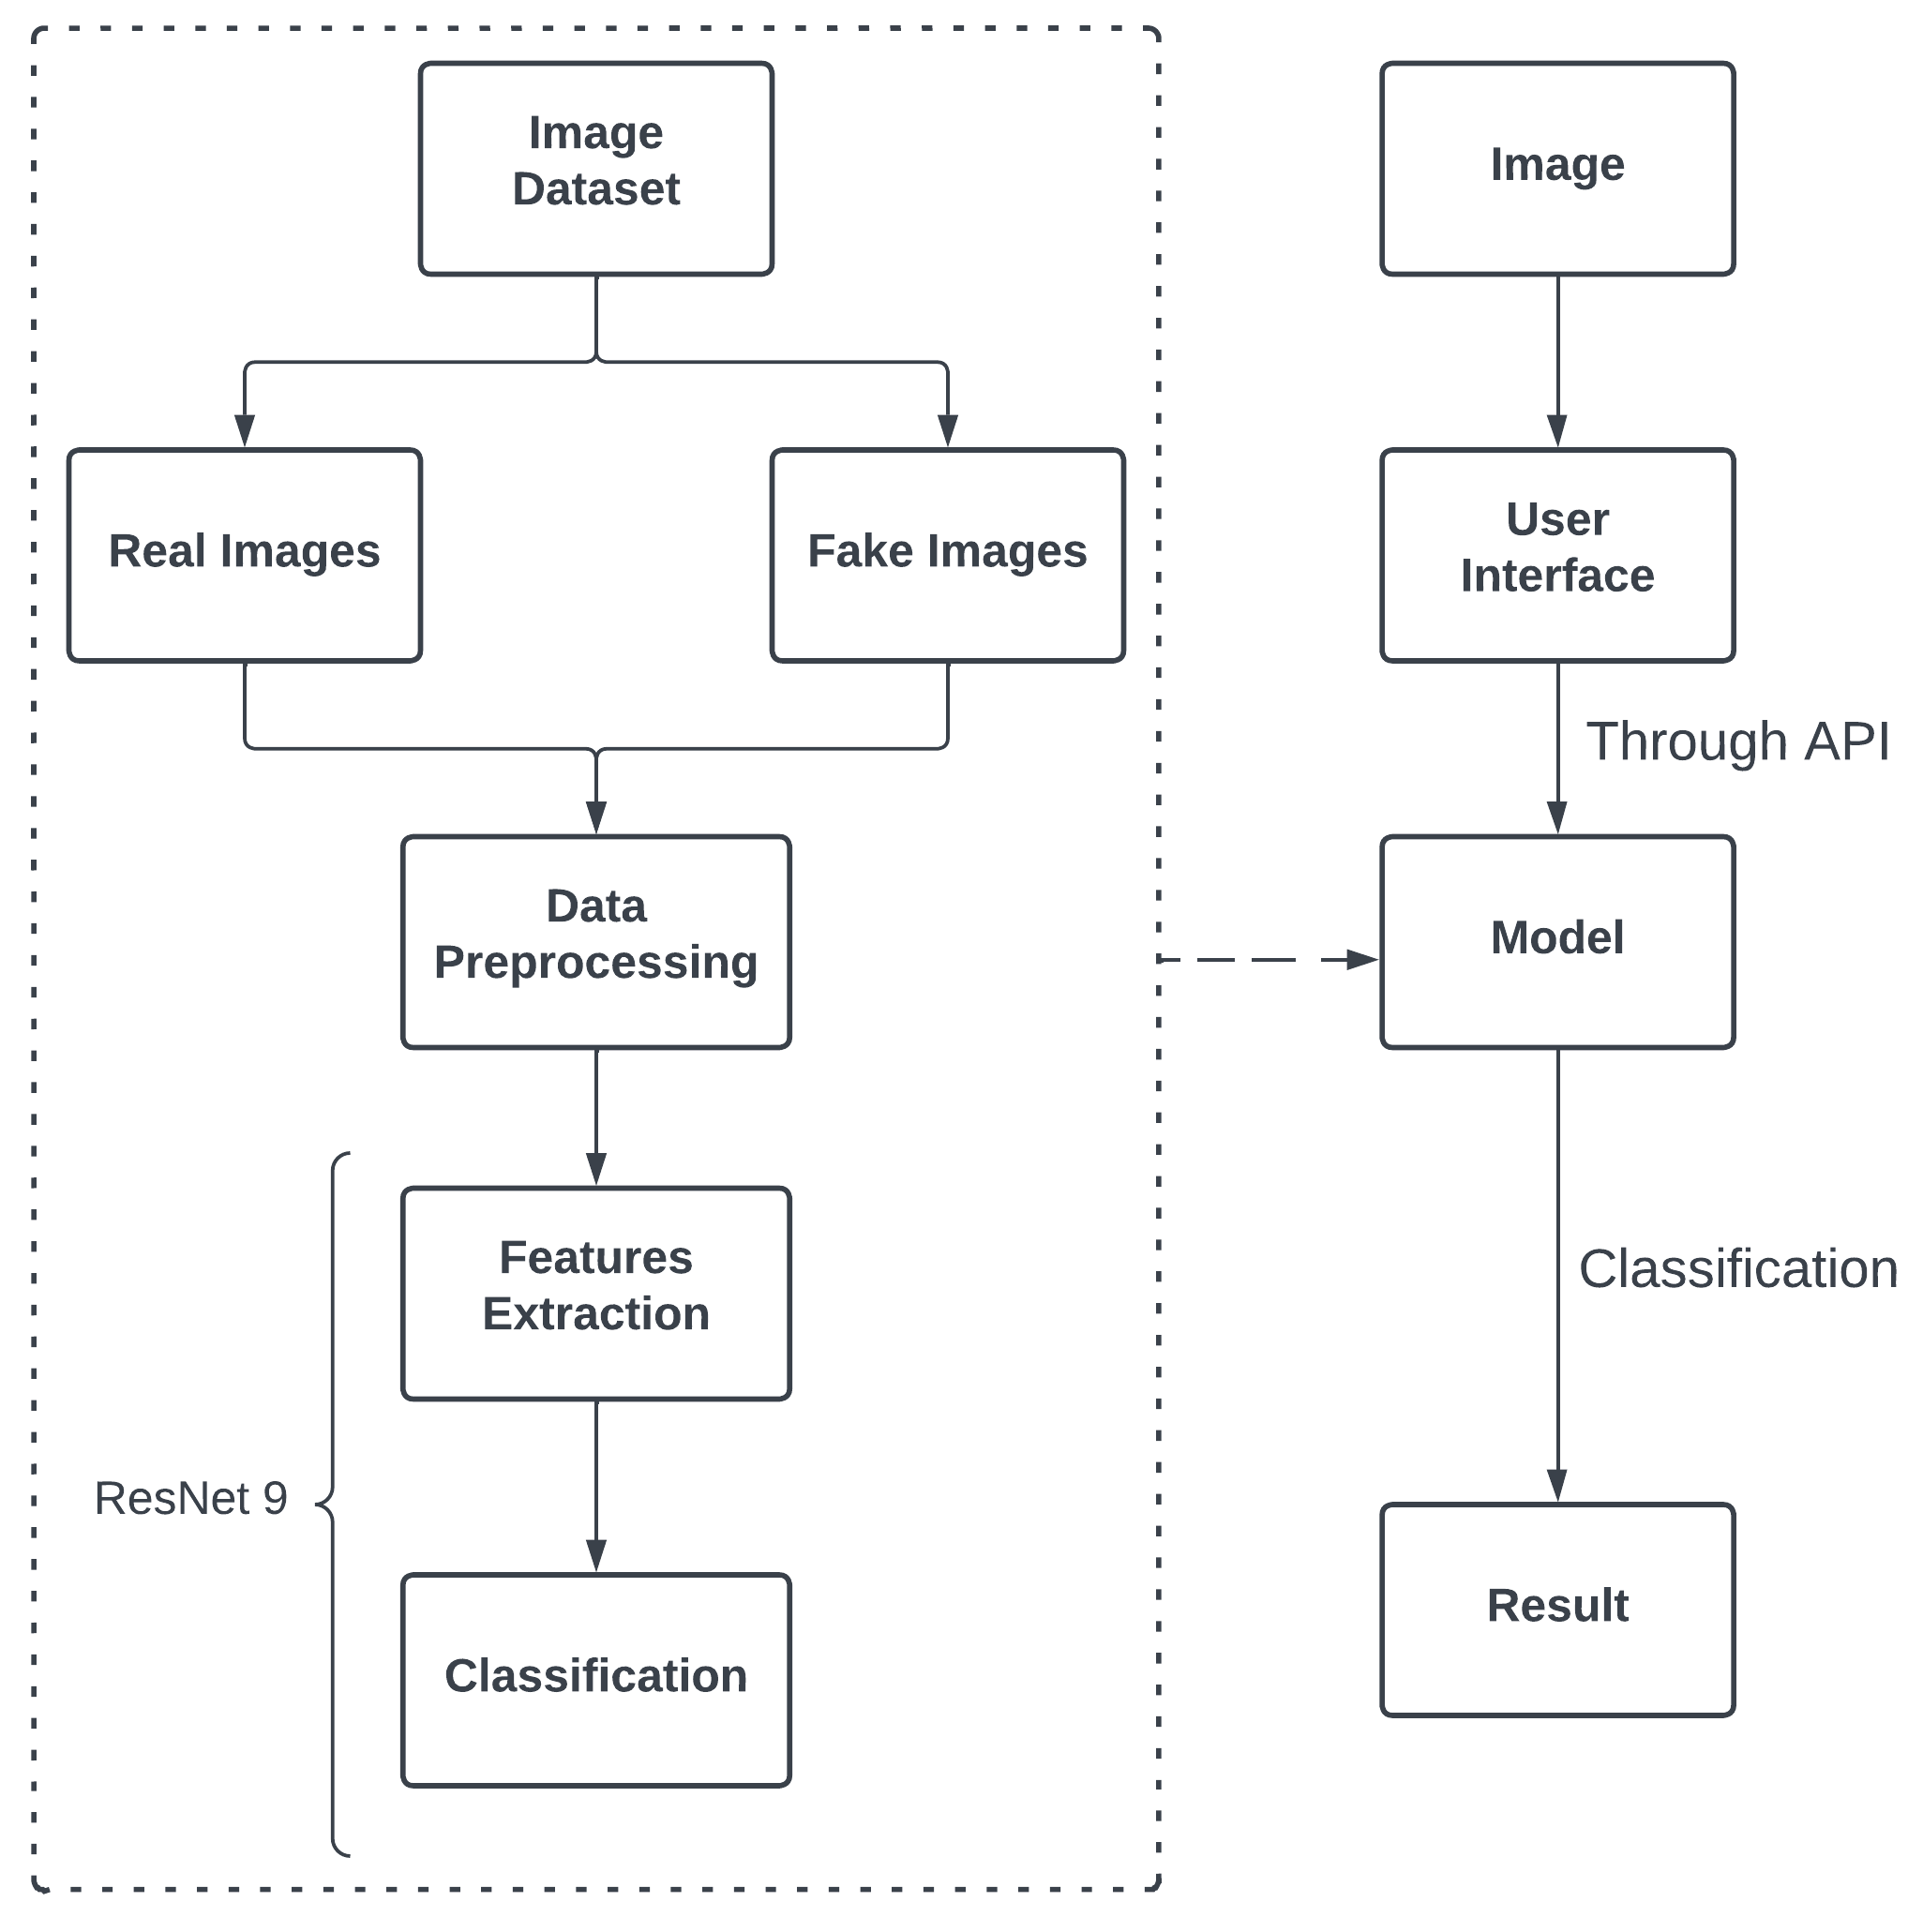
\includegraphics[width=1\textwidth]{./img/Implementation Diagram.png}
        \caption{Block Diagram of Proposed System}
    }
\end{figure}